 \documentclass[10pt, table, dvipsnames, handout]{beamer}
\usetheme[progressbar=frametitle]{metropolis}
\usepackage{appendixnumberbeamer}
\usetikzlibrary{arrows.meta, positioning, quotes}
\usepackage[shortlabels]{enumitem}
\usepackage{xcolor}
\usepackage{mathtools}
\usepackage{dsfont}

\usepackage{cancel}

\newcommand\hcancel[2][black]{\setbox0=\hbox{$#2$}%
\rlap{\raisebox{.45\ht0}{\textcolor{#1}{\rule{\wd0}{1pt}}}}#2} 


\usepackage{booktabs}
\usepackage[scale=2]{ccicons}

\usepackage{pgfplots}
\usepgfplotslibrary{dateplot}

\usepackage{xspace}
\newcommand{\themename}{\textbf{\textsc{metropolis}}\xspace}
\newcommand{\cb}{\cellcolor{blue!25}}


% Notation:
\newcommand{\cT}{\ensuremath{\mathcal{T}}}
\newcommand{\cD}{\ensuremath{\mathcal{D}}}
\newcommand{\cX}{\ensuremath{\mathcal{X}}}
\newcommand{\cY}{\ensuremath{\mathcal{Y}}}
\newcommand{\cZ}{\ensuremath{\mathcal{Z}}}
\newcommand{\cH}{\ensuremath{\mathcal{H}}}

\newcommand{\bR}{\ensuremath{\mathbb{R}}}
\newcommand{\bN}{\ensuremath{\mathbb{N}}}
\newcommand{\bP}{\ensuremath{\mathbb{P}}}
\newcommand{\bT}{\ensuremath{\mathbb{T}}}
\newcommand{\bL}{\ensuremath{\mathbb{L}}}

\newcommand{\bfX}{\ensuremath{\mathbf{X}}}
\newcommand{\bfY}{\ensuremath{\mathbf{Y}}}

\def\layersep{2.5cm}

% Tikz seys
\tikzset{cross/.style={cross out, draw, 
         minimum size=2*(#1-\pgflinewidth), 
         inner sep=0pt, outer sep=0pt}}

\title{Machine Learning I}
\subtitle{Lecture 20: The Vapnik-Chervonenkis Dimension}
% \date{\today}
\date{}
\author{Nathaniel Bade}
\institute{Northeastern University Department of Mathematics}
% \titlegraphic{\hfill\includegraphics[height=1.5cm]{logo.pdf}}

\begin{document}

\maketitle

\begin{frame}{Table of contents}
  \setbeamertemplate{section in toc}[sections numbered]
  \tableofcontents[hideallsubsections]
\end{frame}


%%%%%%%%%%%%%% PAC Learning %%%%%%%%%%%%%% 



\section{Review of Results}

\begin{frame}[fragile]{State of the Union}
The PAC and APAC formalize has provided us a lot to say about the possibility of learning intractable problems. \pause

\textbf{PAC Learning:} For a labeling task, a hypothesis class $\cH$ is \textbf{PAC} learnable if the probability of an ERM learning algorithm being approximately correct can be bounded by the size of the training set, \textit{provided} \textbf{realizability} holds, i.e. some element of $\cH$ provides the labeling, up to a set of measure 0.\pause

\textbf{APAC Learning:} For learning task defined by a loss function and a domain, a hypothesis class $\cH$ is \textbf{APAC} learnable if the probability an ERM learning algorithm returns a classifier with error close to the best error in the hypothesis class can be bounded by the size of the training set.
\end{frame}





\begin{frame}[fragile]{State of the Union}
Over the last lectures, we proved that several hypothesis classes were, respectively, PAC and APAC learnable:\pause


\textbf{PAC Learnable:} The (infinite) class of interval indicator functions is PAC learnable, with sample complexity
$$
N_\cH(\epsilon,\delta) \leq \text{ceil}\left(\, \frac{2\log (2/\delta)}{\epsilon}\,\right)\,.
$$
\pause

\textbf{APAC Learnable:} Any finite hypothesis class $\cH$ is APAC learnable, with sample complexity
$$
N_\cH(\epsilon,\delta) \leq \text{ceil}\left(\, \frac{2\log (2|\cH|/\delta)}{\epsilon^2}\,\right)\,.
$$
\end{frame}




\begin{frame}[fragile]{State of the Union}
The examples before show that there are infinite classes of functions that are PAC learnable and finite classes of functions that APAC learnable. This raises a few questions:

\begin{itemize}
\item[] Are PAC learnable classes APAC learnable?\pause
\item[] Are \emph{all} classes PAC learnable?\pause
\item[] Is there an efficient way to tell if a class is PAC/APAC learnable?\pause
\end{itemize}
We will answer all these questions this lecture. \pause The most surprising might be that the we can answer the first question in the affirmative. {\color{white} But what is an example of an unlearnable class?}

\end{frame}



\begin{frame}[fragile]{State of the Union}
The examples before show that there are infinite classes of functions that are PAC learnable and finite classes of functions that APAC learnable. This raises a few questions:

\begin{itemize}
\item[] Are PAC learnable classes APAC learnable? \textbf{Yes, surprisingly.}
\item[] Are \emph{all} classes PAC learnable? \textbf{No.}
\item[] Is there a easy way to tell if a class is PAC/APAC learnable? \textbf{Yes.}
\end{itemize}
We will answer all these questions this lecture. The most surprising might be that the we can answer the second question in the affirmative. \pause  But what is an example of an unlearnable class?

\end{frame}



\section{The class of all functions is unlearnable.}



\begin{frame}[fragile]{No Free Lunch}
Recall that we also proved

\textbf{No Free Lunch Theorem:} For any learning algorithm for the task of binary classification with respect to the 0-1 loss function, provided the training size $\cT$ is less than $|\cX|/2$, there exists a learnable distribution $\cD$ over $\cX\times \{0,1\}$ such that 
$$
L_\cD(A(\cT)) \geq 1/8
$$
with probability 1/7. \pause That is any learning algorithm $A$ and any class $\cH$ has a learnable task at which they do poorly. \pause 

This gives us a direct proof of the fact that the class of all functions is unlearnable.
\end{frame}





\begin{frame}[fragile]{PAC Unlearnable}
\textbf{(SB - Corollary 5.2)} Let $\cX$ be an infinite domain set and let $\cH_{all}$ be the set of all functions from $\cX$ to $\{0,1\}$. Then $\cH$ is not PAC learnable.\pause\newline

\textbf{Proof:} Assume $\cH_{all}$ is PAC learnable by a algorithm $A$. \pause By the No Free Lunch theorem, there is some distribution $\cD$ on $\cX\times\{0,1\}$ and some function $f:\cX\to \{0,1\}$ such that $L_\cD(f) = 0$, and $L_\cD(A(\cT))>1/8$ with probability greater than $1/7$. \pause

However, the existence of an $f$ such that $L_\cD(f) = 0$ means $\cH_{all}$ is realizable. \pause That implies that for any $ \delta<1/7$ and $\epsilon<1/8$, there exists an $N$ such that if $|\cT|>N$, $L_\cD(A(f))<\epsilon.$ \pause 

This is a contradiction, so $\cH_{all}$ is not PAC learnable. 

\hspace*{\fill} $\Box$
\end{frame}







\begin{frame}[fragile]{PAC Unlearnable}
  \begin{minipage}[t][0.6\textheight][t]{\textwidth}
	\centering \includegraphics[height=0.6\textheight]{L6LinearClass2.png} 
  \end{minipage}
  \vfill
  \begin{minipage}[t][0.4\textheight][t]{\textwidth}
\textbf{Question:} Why doesn't this proof imply that \textbf{no} function is PAC learnable? \newline

\only<2| handout:0>{The key is the fact that any deterministic labeling makes $\cH_{all}$ realizable, so the minimum possible error over $\cH_{all}$ must be 0. For the linear classifier, a sufficiently bad distribution is simply not realizable.}

\only<3| handout:0>{For example, we know that a linear classifier does badly on some learnable sets. PAC learnability only says it should do well if the labeling is generated by a linear classifier.}
\end{minipage}

\end{frame}








\section{The VC Dimension}




\begin{frame}[fragile]{VC Dimension}
We have seen that finiteness is a sufficient criteria for learnability. We have also seen that while some infinite classes are PAC learnable some infinite classes are not. In other words, the cardinality of $\cH$ isn't the proper decider of learnability. \pause

We will show that a property called the VC-dimension of a hypothesis class gives the correct characterization of (A)PAC learnability. To motivate VC-dimension, lets recall a bit about how we proved the No Free Lunch Theorem.

\end{frame}



\begin{frame}[fragile]{No Free Lunch Arguments}
  \begin{minipage}[t][0.6\textheight][t]{\textwidth}
	\centering \includegraphics[height=0.6\textheight]{L6LinearClass2.png} 
  \end{minipage}
  \vfill
  \begin{minipage}[t][0.4\textheight][t]{\textwidth}
The idea of the proof was to construct a distribution $\mathcal{D}$ on which the learning algorithm would perform poorly.
\end{minipage}

\end{frame}




\begin{frame}[fragile]{No Free Lunch Arguments}
  \begin{minipage}[t][0.6\textheight][t]{\textwidth}
	\centering \includegraphics[height=0.6\textheight]{L6LinearLabeling3.png} 
  \end{minipage}
  \vfill
  \begin{minipage}[t][0.4\textheight][t]{\textwidth}
The idea of the proof was to construct an distribution $\mathcal{D}$ on which the learning algorithm would perform poorly. \pause We defined a class of distributions concentrated on a finite set $C\subseteq \cX$ with a deterministic "true" labeling function $f$ chosen from the set of all functions. 
\end{minipage}

\end{frame}


\begin{frame}[fragile]{No Free Lunch Arguments}
  \begin{minipage}[t][0.6\textheight][t]{\textwidth}
	\centering \includegraphics[height=0.6\textheight]{L6LinearLabeling4.png} 
  \end{minipage}
  \vfill
  \begin{minipage}[t][0.4\textheight][t]{\textwidth}
The idea of the proof was to construct an distribution $\mathcal{D}$ on which the learning algorithm would perform poorly. \pause We defined a class of distributions concentrated on a finite set $C\subseteq \cX$ with a deterministic "true" labeling function $f$ chosen from the set of all functions. 
\end{minipage}

\end{frame}



\begin{frame}[fragile]{No Free Lunch Arguments}
  \begin{minipage}[t][0.6\textheight][t]{\textwidth}
	\centering \includegraphics[height=0.6\textheight]{L6LinearLabeling5.png} 
  \end{minipage}
  \vfill
  \begin{minipage}[t][0.4\textheight][t]{\textwidth}
The idea of the proof was to construct an distribution $\mathcal{D}$ on which the learning algorithm would perform poorly. \pause We defined a class of distributions concentrated on a finite set $C\subseteq \cX$ with a deterministic "true" labeling function $f$ chosen from the set of all functions. 
\end{minipage}

\end{frame}



\begin{frame}[fragile]{No Free Lunch Arguments}
  \begin{minipage}[t][0.6\textheight][t]{\textwidth}
	\centering \includegraphics[height=0.6\textheight]{L6LinearLabeling6.png} 
  \end{minipage}
  \vfill
  \begin{minipage}[t][0.4\textheight][t]{\textwidth}
To make an algorithm fail, we used the fact that we could pick a labeling from the set of all possible functions from $C\to \{0,1\}$. 
\end{minipage}

\end{frame}



\begin{frame}[fragile]{No Free Lunch Arguments}
  \begin{minipage}[t][0.6\textheight][t]{\textwidth}
	\centering \includegraphics[height=0.6\textheight]{L6LinearLabeling7.png} 
  \end{minipage}
  \vfill
  \begin{minipage}[t][0.4\textheight][t]{\textwidth}
To make the algorithm fail, we used the fact that we could pick a labeling from the set of all possible functions from $C\to \{0,1\}$. We saw there was then a high probability that a random training sample will produce a "bad" classifier. 
\end{minipage}

\end{frame}




\begin{frame}[fragile]{No Free Lunch Arguments}
  \begin{minipage}[t][0.6\textheight][t]{\textwidth}
	\centering \includegraphics[height=0.6\textheight]{L6LinearLabeling5.png} 
  \end{minipage}
  \vfill
  \begin{minipage}[t][0.4\textheight][t]{\textwidth}
When considering PAC learnability, realizability restricts the distribution to only the ones for which some hypothesis in $\cH$ achieves zero risk. \pause So if $\cH$ restricted to $C$ is the set of all functions, we can construct a \textbf{realizable} distribution that $\cH$ must fail to learn. \pause If $\cH$ restricted to $C$ is not the set of all functions, we have a hope $\cH$ is learnable for all realizable tasks. 
\end{minipage}

\end{frame}




\begin{frame}[fragile]{Restricting}
\textbf{The restriction of $\cH$ to $C$.} Let $\cH$ be a hypothesis class of functions from $\cX\to \{0,1\}$ and let 
$$
C = \{c_1,\ldots, c_m\}\subset \cX
$$
be a finite subset of $\cX$. \pause The \textbf{restriction} of $\cH$ to $C$ is the set of all function from $C$ to $\{0,1\}$ that can be derived from $\cH$:
$$
\cH_C = \big\{\,\big(\,h(c_1),\ldots,h(c_m)\,\big) : h\in \cH\}\,.
$$\pause

If the restriction of $\cH$ to $C$ is the set of all function, we say $\cH$ \textbf{shatters} $C$. 
\end{frame}





\begin{frame}[fragile]{Shattering for Linear Classifier}
  \begin{minipage}[t][0.6\textheight][t]{\textwidth}
	\centering \includegraphics[height=0.6\textheight]{L6Shattering1.png} 
  \end{minipage}
  \vfill
  \begin{minipage}[t][0.4\textheight][t]{\textwidth}
A hypothesis class \textbf{shatters} a finite set $C\subset\cX$ if the restriction of $\cH$ to $C$ is the set of all functions. \pause

For example, the 3 point set can be shattered by the halfplane classifier, since any labeling on the three points can be generated by a half plane.
\end{minipage}

\end{frame}





\begin{frame}[fragile]{Shattering for Linear Classifier}
  \begin{minipage}[t][0.6\textheight][t]{\textwidth}
	\centering \includegraphics[height=0.6\textheight]{L6Shattering2.png} 
  \end{minipage}
  \vfill
  \begin{minipage}[t][0.4\textheight][t]{\textwidth}
Formally, a hypothesis class \textbf{shatters} a finite set $C\subset\cX$ if the restriction of $\cH$ to $C$ is the set of all functions. 

For example, the 3 point set can be shattered by the halfplane classifier, since any labeling on the three points can be generated by a half plane.
\end{minipage}

\end{frame}




\begin{frame}[fragile]{Shattering for Linear Classifier}
  \begin{minipage}[t][0.6\textheight][t]{\textwidth}
	\centering \includegraphics[height=0.6\textheight]{L6Shattering3.png} 
  \end{minipage}
  \vfill
  \begin{minipage}[t][0.4\textheight][t]{\textwidth}
Formally, a hypothesis class \textbf{shatters} a finite set $C\subset\cX$ if the restriction of $\cH$ to $C$ is the set of all functions. 

For example, the 3 point set can be shattered by the halfplane classifier, since any labeling on the three points can be generated by a half plane.
\end{minipage}

\end{frame}



\begin{frame}[fragile]{Shattering for Linear Classifier}
  \begin{minipage}[t][0.6\textheight][t]{\textwidth}
	\centering \includegraphics[height=0.6\textheight]{L6Shattering4.png} 
  \end{minipage}
  \vfill
  \begin{minipage}[t][0.4\textheight][t]{\textwidth}
Formally, a hypothesis class \textbf{shatters} a finite set $C\subset\cX$ if the restriction of $\cH$ to $C$ is the set of all functions. 

For example, the 3 point set can be shattered by the halfplane classifier, since any labeling on the three points can be generated by a half plane.
\end{minipage}

\end{frame}



\begin{frame}[fragile]{Shattering for Linear Classifier}
  \begin{minipage}[t][0.6\textheight][t]{\textwidth}
	\centering \includegraphics[height=0.6\textheight]{L6Shattering5.png} 
  \end{minipage}
  \vfill
  \begin{minipage}[t][0.4\textheight][t]{\textwidth}
Formally, a hypothesis class \textbf{shatters} a finite set $C\subset\cX$ if the restriction of $\cH$ to $C$ is the set of all functions. 

For example, the 3 point set can be shattered by the halfplane classifier, since any labeling on the three points can be generated by a half plane.
\end{minipage}

\end{frame}



\begin{frame}[fragile]{Shattering for Linear Classifier}
  \begin{minipage}[t][0.6\textheight][t]{\textwidth}
	\centering \includegraphics[height=0.6\textheight]{L6Shattering6.png} 
  \end{minipage}
  \vfill
  \begin{minipage}[t][0.4\textheight][t]{\textwidth}
Formally, a hypothesis class \textbf{shatters} a finite set $C\subset\cX$ if the restriction of $\cH$ to $C$ is the set of all functions. 

For example, the 3 point set can be shattered by the halfplane classifier, since any labeling on the three points can be generated by a half plane.
\end{minipage}

\end{frame}


\begin{frame}[fragile]{Shattering for Linear Classifier}
  \begin{minipage}[t][0.6\textheight][t]{\textwidth}
	\centering \includegraphics[height=0.6\textheight]{L6Shattering7.png} 
  \end{minipage}
  \vfill
  \begin{minipage}[t][0.4\textheight][t]{\textwidth}
Formally, a hypothesis class \textbf{shatters} a finite set $C\subset\cX$ if the restriction of $\cH$ to $C$ is the set of all functions. 

For example, the 3 point set can be shattered by the halfplane classifier, since any labeling on the three points can be generated by a half plane.
\end{minipage}

\end{frame}


\begin{frame}[fragile]{Shattering for Linear Classifier}
  \begin{minipage}[t][0.6\textheight][t]{\textwidth}
	\centering \includegraphics[height=0.6\textheight]{L6Shattering8.png} 
  \end{minipage}
  \vfill
  \begin{minipage}[t][0.4\textheight][t]{\textwidth}
Formally, a hypothesis class \textbf{shatters} a finite set $C\subset\cX$ if the restriction of $\cH$ to $C$ is the set of all functions. 

For example, the 3 point set can be shattered by the halfplane classifier, since any labeling on the three points can be generated by a half plane.
\end{minipage}

\end{frame}




\begin{frame}[fragile]{Shattering for Linear Classifier}
  \begin{minipage}[t][0.6\textheight][t]{\textwidth}
	\centering \includegraphics[height=0.6\textheight]{L6Shattering8.png} 
  \end{minipage}
  \vfill
  \begin{minipage}[t][0.4\textheight][t]{\textwidth}
This means that for a training set of size $N = \text{floor}(\frac32)$, we can construct a distribution on 3 points that is unlearnable by the set of half plane classifiers.  

\end{minipage}

\end{frame}





\begin{frame}[fragile]{Shattering for Linear Classifier}
  \begin{minipage}[t][0.6\textheight][t]{\textwidth}
	\centering \includegraphics[height=0.6\textheight]{L6Shattering9.png} 
  \end{minipage}
  \vfill
  \begin{minipage}[t][0.4\textheight][t]{\textwidth}
On the other hand, the restriction of the halfplane classifiers to any 4 point set $C$ is not the set of all functions from $C\to \{0,1\}$. \pause Four point sets come in two configurations, a point inside the convex hull of three points, 

\end{minipage}

\end{frame}




\begin{frame}[fragile]{Shattering for Linear Classifier}
  \begin{minipage}[t][0.6\textheight][t]{\textwidth}
	\centering \includegraphics[height=0.6\textheight]{L6Shattering10.png} 
  \end{minipage}
  \vfill
  \begin{minipage}[t][0.4\textheight][t]{\textwidth}
On the other hand, the restriction of the halfplane classifiers to any 4 point set $C$ is not the set of the functions  from $C\to \{0,1\}$. Four point sets come in two configurations, a point inside the convex hull of three points, and a convex four polygone. \pause In both cases, there are labelings that cannot be determined by a halfplane classifier. 
\end{minipage}

\end{frame}









\begin{frame}[fragile]{Shattering and No Free Lunch}\
Putting this reasoning together, we have

\textbf{(SB - Theorem 6.6)} Let $\cH$ be a hypothesis class of functions $\cX\to\{0,1\}$ and $N$ be a training set size. \pause Assume there exists a set $C\subset \cX$ of size $2N$ that is shattered by $\cH$. \pause 

For any learning algorithm $A$,  there exists a distribution $\cD$ over $\cX\times\{0,1\}$ and a predictor $h\in \cH$ such that $L_\cD(h) = 0$, but with probability at least 1/7 over the choice of training sets $\cT$, 
$$
L_\cD(A(\cT))\geq 1/8\,.
$$\pause

In other words, if $\cH$ shatters a set $C$ of size $2N$, we cant learn learn $\cH$ using $N$ examples. 


\end{frame}



\begin{frame}[fragile]{Shattering and No Free Lunch}
  \begin{minipage}[t][0.6\textheight][t]{\textwidth}
	\centering \includegraphics[height=0.6\textheight]{hexagon.jpg} 
  \end{minipage}
  \vfill
  \begin{minipage}[t][0.4\textheight][t]{\textwidth}
  
The author Borges has a story about an infinite library which contains a book with ever possible combination of letters. Somewhere in the library, books every truth must be lie but they are impossible to find, and the librarians spend their lives contending with gibberish. 
\end{minipage}
\end{frame}



\begin{frame}[fragile]{Shattering and No Free Lunch}
  \begin{minipage}[t][0.6\textheight][t]{\textwidth}
	\centering \includegraphics[height=0.6\textheight]{hexagon.jpg} 
  \end{minipage}
  \vfill
  \begin{minipage}[t][0.4\textheight][t]{\textwidth}
  
Philosophically, if a hypothesis class knows every labeling then, like Borges' library, any truth must be contained somewhere in it but will be impossible to find.
\end{minipage}
\end{frame}




\begin{frame}[fragile]{VC-Dimension}
This lead us directly to the following definition: The \textbf{VC-dimension} of a hypothesis class, denoted $\text{VCDim}(\cH)$ is the maximum size of a set that can be shattered by $\cH$. If $\cH$ can shatter sets of arbitrary size, we say it has infinite VC-dimension. \pause\newline

\textbf{SB Theorem 6.6:} If $\cH$ is a class of infinite VC-dimension, then $\cH$ is not PAC learnable. \pause\newline

\textbf{Proof:} Since $\cH$ has infinite VC-dimension, for any $N$ there is a set of size $2N$ shattered by $\cH$. $\Box$ \pause \newline

We shall see later that if $\cH$ has finite VC-dimension it is PAC learnable.
\end{frame}





\section{Examples of VC Dimension}


\begin{frame}[fragile]{VC-Dimension}
  \begin{minipage}[t][0.5\textheight][t]{\textwidth}
	\centering
	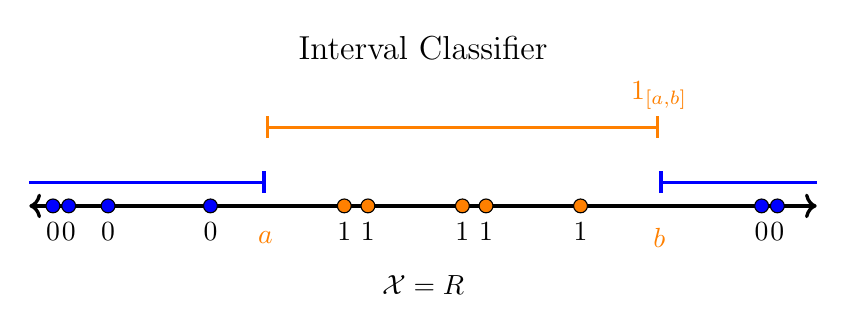
\begin{tikzpicture}
		\draw[<->,very thick] (-5,0) -- (5,0);
		\draw[color = orange, |-|,very thick] (-2,1) -- (3,1);
		\draw[color=blue, -|,very thick] (-5,.3)--(-2,.3);
		\draw[color=blue, |-,very thick] (3,.3)--(5,.3);
		\node[color=orange] at (3,1.4) {$1_{[a,b]}$};
		\node at (0,2) {\large Interval Classifier} ;
		\node at (0,-1) {$\mathcal{X} = \mathbb{R}$} ;

		\node [color=orange] at (-2,-.4) {$a$} ;
		\node [color=orange] at (3,-.4) {$b$} ;

%		\draw [color=olive, |-|,very thick] (-3.5,0) -- (2.5,0);
%		\node [color=olive] at (3,.4) {$h_{\mathcal{T}}$} ;



		\node[circle,draw=black, fill=orange, inner sep=0pt,minimum size=5pt, label=below:1] at (2,0) {};
		\node[circle,draw=black, fill=orange, inner sep=0pt,minimum size=5pt, label=below:1] at (-1,0) {};
		\node[circle,draw=black, fill=orange, inner sep=0pt,minimum size=5pt, label=below:1] at (-.7,0) {};
		\node[circle,draw=black, fill=orange, inner sep=0pt,minimum size=5pt, label=below:1] at (.5,0) {};
		\node[circle,draw=black, fill=orange, inner sep=0pt,minimum size=5pt, label=below:1] at (.8,0) {};
%		\node[circle,draw=black, fill=orange, inner sep=0pt,minimum size=5pt, label=below:1] at (3.5,0) {};

		\node[circle,draw=black, fill=blue, inner sep=0pt,minimum size=5pt, label=below:0] at (-2.7,0) {};
		\node[circle,draw=black, fill=blue, inner sep=0pt,minimum size=5pt, label=below:0] at (-4.5,0) {};
		\node[circle,draw=black, fill=blue, inner sep=0pt,minimum size=5pt, label=below:0] at (-4,0) {};
		\node[circle,draw=black, fill=blue, inner sep=0pt,minimum size=5pt, label=below:0] at (-4.7,0) {};
		\node[circle,draw=black, fill=blue, inner sep=0pt,minimum size=5pt, label=below:0] at (4.3,0) {};
		\node[circle,draw=black, fill=blue, inner sep=0pt,minimum size=5pt, label=below:0] at (4.5,0) {};
	\end{tikzpicture}
  \end{minipage}
  \vfill
  \begin{minipage}[t][0.5\textheight][t]{\textwidth}
\textbf{Question:} What is the VC-dimension of the hypothesis class of interval classifiers $1_{[a,b]}$ on $\bR$?


\end{minipage}
\end{frame}


\begin{frame}<handout:0>[fragile]{VC-Dimension}
  \begin{minipage}[t][0.5\textheight][t]{\textwidth}
	\centering
	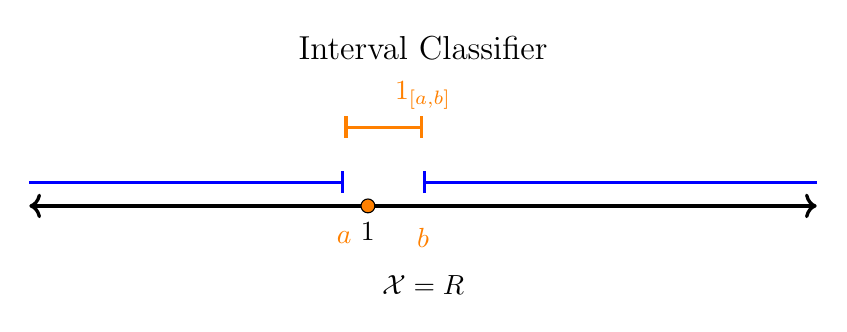
\begin{tikzpicture}
		\def\le{-1}
		\def\re{0}
		\draw[<->,very thick] (-5,0) -- (5,0);
		\draw[color = orange, |-|,very thick] (\le,1) -- (\re,1);
		\draw[color=blue, -|,very thick] (-5,.3)--(\le,.3);
		\draw[color=blue, |-,very thick] (\re,.3)--(5,.3);
		\node[color=orange] at (\re,1.4) {$1_{[a,b]}$};
		\node at (0,2) {\large Interval Classifier} ;
		\node at (0,-1) {$\mathcal{X} = \mathbb{R}$} ;

		\node [color=orange] at (\le,-.4) {$a$} ;
		\node [color=orange] at (\re,-.4) {$b$} ;

		\node[circle,draw=black, fill=orange, inner sep=0pt,minimum size=5pt, label=below:1] at (-.7,0) {};
	\end{tikzpicture}
  \end{minipage}
  \vfill
  \begin{minipage}[t][0.5\textheight][t]{\textwidth}
\textbf{Question:} What is the VC-dimension of the hypothesis class of interval classifiers $1_{[a,b]}$ on $\bR$?\newline

The class $\cH$ can clearly shatter a single point.


\end{minipage}
\end{frame}


\begin{frame}<handout:0>[fragile]{VC-Dimension}
  \begin{minipage}[t][0.5\textheight][t]{\textwidth}
	\centering
	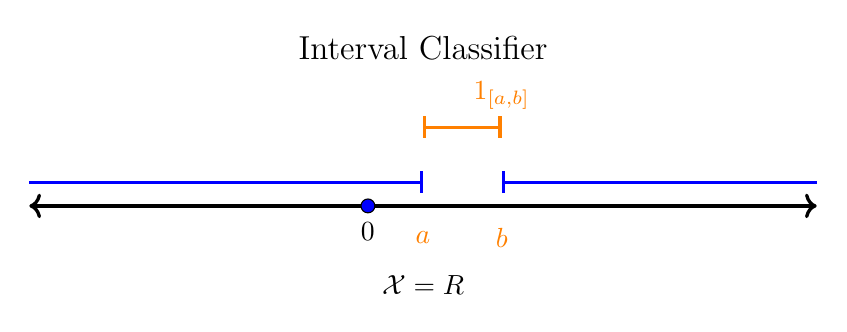
\begin{tikzpicture}
		\def\le{0}
		\def\re{1}
		\draw[<->,very thick] (-5,0) -- (5,0);
		\draw[color = orange, |-|,very thick] (\le,1) -- (\re,1);
		\draw[color=blue, -|,very thick] (-5,.3)--(\le,.3);
		\draw[color=blue, |-,very thick] (\re,.3)--(5,.3);
		\node[color=orange] at (\re,1.4) {$1_{[a,b]}$};
		\node at (0,2) {\large Interval Classifier} ;
		\node at (0,-1) {$\mathcal{X} = \mathbb{R}$} ;

		\node [color=orange] at (\le,-.4) {$a$} ;
		\node [color=orange] at (\re,-.4) {$b$} ;

		\node[circle,draw=black, fill=blue, inner sep=0pt,minimum size=5pt, label=below:0] at (-.7,0) {};
	\end{tikzpicture}
  \end{minipage}
  \vfill
  \begin{minipage}[t][0.5\textheight][t]{\textwidth}
\textbf{Question:} What is the VC-dimension of the hypothesis class of interval classifiers $1_{[a,b]}$ on $\bR$?\newline

The class $\cH$ can clearly shatter a single point.


\end{minipage}
\end{frame}









\begin{frame}<handout:0>[fragile]{VC-Dimension}
  \begin{minipage}[t][0.5\textheight][t]{\textwidth}
	\centering
	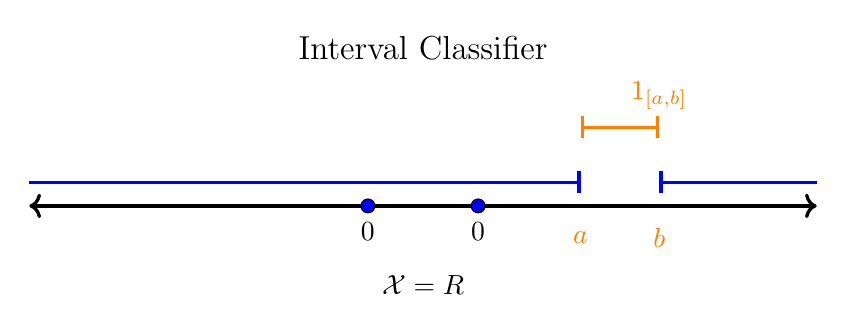
\begin{tikzpicture}
		\def\le{2}
		\def\re{3}
		\draw[<->,very thick] (-5,0) -- (5,0);
		\draw[color = orange, |-|,very thick] (\le,1) -- (\re,1);
		\draw[color=blue, -|,very thick] (-5,.3)--(\le,.3);
		\draw[color=blue, |-,very thick] (\re,.3)--(5,.3);
		\node[color=orange] at (\re,1.4) {$1_{[a,b]}$};
		\node at (0,2) {\large Interval Classifier} ;
		\node at (0,-1) {$\mathcal{X} = \mathbb{R}$} ;

		\node [color=orange] at (\le,-.4) {$a$} ;
		\node [color=orange] at (\re,-.4) {$b$} ;

		\node[circle,draw=black, fill=blue, inner sep=0pt,minimum size=5pt, label=below:0] at (-.7,0) {};
		\node[circle,draw=black, fill=blue, inner sep=0pt,minimum size=5pt, label=below:0] at (.7,0) {};
	\end{tikzpicture}
  \end{minipage}
  \vfill
  \begin{minipage}[t][0.5\textheight][t]{\textwidth}
\textbf{Question:} What is the VC-dimension of the hypothesis class of interval classifiers $1_{[a,b]}$ on $\bR$?\newline

The class $\cH$ can clearly shatter a single point. It can also shatter a two point set.

\end{minipage}
\end{frame}



\begin{frame}<handout:0>[fragile]{VC-Dimension}
  \begin{minipage}[t][0.5\textheight][t]{\textwidth}
	\centering
	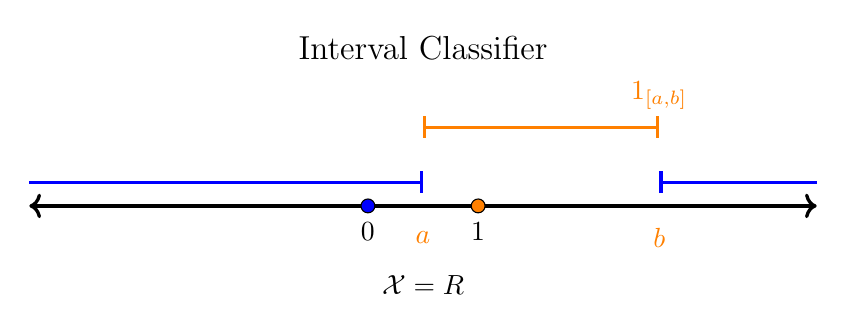
\begin{tikzpicture}
		\def\le{0}
		\def\re{3}
		\draw[<->,very thick] (-5,0) -- (5,0);
		\draw[color = orange, |-|,very thick] (\le,1) -- (\re,1);
		\draw[color=blue, -|,very thick] (-5,.3)--(\le,.3);
		\draw[color=blue, |-,very thick] (\re,.3)--(5,.3);
		\node[color=orange] at (\re,1.4) {$1_{[a,b]}$};
		\node at (0,2) {\large Interval Classifier} ;
		\node at (0,-1) {$\mathcal{X} = \mathbb{R}$} ;

		\node [color=orange] at (\le,-.4) {$a$} ;
		\node [color=orange] at (\re,-.4) {$b$} ;

		\node[circle,draw=black, fill=blue, inner sep=0pt,minimum size=5pt, label=below:0] at (-.7,0) {};
		\node[circle,draw=black, fill=orange, inner sep=0pt,minimum size=5pt, label=below:1] at (.7,0) {};
	\end{tikzpicture}
  \end{minipage}
  \vfill
  \begin{minipage}[t][0.5\textheight][t]{\textwidth}
\textbf{Question:} What is the VC-dimension of the hypothesis class of interval classifiers $1_{[a,b]}$ on $\bR$?\newline

The class $\cH$ can clearly shatter a single point. It can also shatter a two point set.

\end{minipage}
\end{frame}




\begin{frame}<handout:0>[fragile]{VC-Dimension}
  \begin{minipage}[t][0.5\textheight][t]{\textwidth}
	\centering
	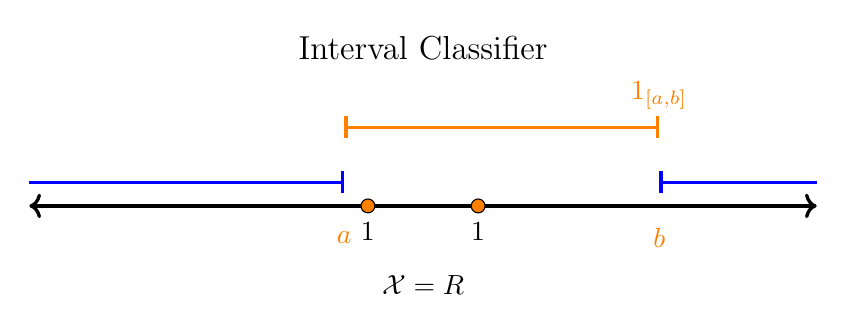
\begin{tikzpicture}
		\def\le{-1}
		\def\re{3}
		\draw[<->,very thick] (-5,0) -- (5,0);
		\draw[color = orange, |-|,very thick] (\le,1) -- (\re,1);
		\draw[color=blue, -|,very thick] (-5,.3)--(\le,.3);
		\draw[color=blue, |-,very thick] (\re,.3)--(5,.3);
		\node[color=orange] at (\re,1.4) {$1_{[a,b]}$};
		\node at (0,2) {\large Interval Classifier} ;
		\node at (0,-1) {$\mathcal{X} = \mathbb{R}$} ;

		\node [color=orange] at (\le,-.4) {$a$} ;
		\node [color=orange] at (\re,-.4) {$b$} ;

		\node[circle,draw=black, fill=orange, inner sep=0pt,minimum size=5pt, label=below:1] at (-.7,0) {};
		\node[circle,draw=black, fill=orange, inner sep=0pt,minimum size=5pt, label=below:1] at (.7,0) {};
	\end{tikzpicture}
  \end{minipage}
  \vfill
  \begin{minipage}[t][0.5\textheight][t]{\textwidth}
\textbf{Question:} What is the VC-dimension of the hypothesis class of interval classifiers $1_{[a,b]}$ on $\bR$?\newline

The class $\cH$ can clearly shatter a single point. It can also shatter a two point set.

\end{minipage}
\end{frame}




\begin{frame}<handout:0>[fragile]{VC-Dimension}
  \begin{minipage}[t][0.5\textheight][t]{\textwidth}
	\centering
	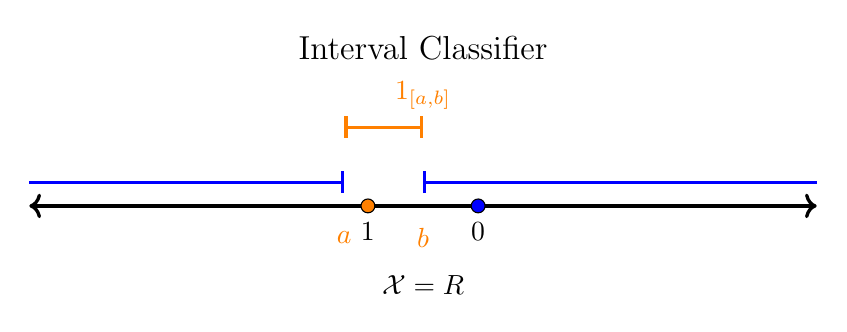
\begin{tikzpicture}
		\def\le{-1}
		\def\re{0}
		\draw[<->,very thick] (-5,0) -- (5,0);
		\draw[color = orange, |-|,very thick] (\le,1) -- (\re,1);
		\draw[color=blue, -|,very thick] (-5,.3)--(\le,.3);
		\draw[color=blue, |-,very thick] (\re,.3)--(5,.3);
		\node[color=orange] at (\re,1.4) {$1_{[a,b]}$};
		\node at (0,2) {\large Interval Classifier} ;
		\node at (0,-1) {$\mathcal{X} = \mathbb{R}$} ;

		\node [color=orange] at (\le,-.4) {$a$} ;
		\node [color=orange] at (\re,-.4) {$b$} ;

		\node[circle,draw=black, fill=orange, inner sep=0pt,minimum size=5pt, label=below:1] at (-.7,0) {};
		\node[circle,draw=black, fill=blue, inner sep=0pt,minimum size=5pt, label=below:0] at (.7,0) {};
	\end{tikzpicture}
  \end{minipage}
  \vfill
  \begin{minipage}[t][0.5\textheight][t]{\textwidth}
\textbf{Question:} What is the VC-dimension of the hypothesis class of interval classifiers $1_{[a,b]}$ on $\bR$?\newline

The class $\cH$ can clearly shatter a single point. It can also shatter a two point set.

\end{minipage}
\end{frame}








\begin{frame}<handout:0>[fragile]{VC-Dimension}
  \begin{minipage}[t][0.5\textheight][t]{\textwidth}
	\centering
	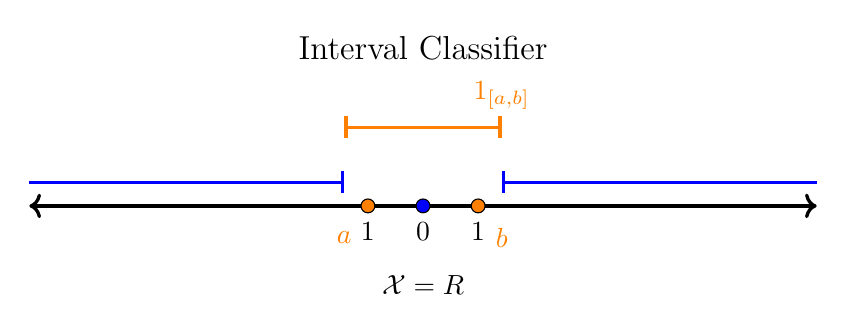
\begin{tikzpicture}
		\def\le{-1}
		\def\re{1}
		\draw[<->,very thick] (-5,0) -- (5,0);
		\draw[color = orange, |-|,very thick] (\le,1) -- (\re,1);
		\draw[color=blue, -|,very thick] (-5,.3)--(\le,.3);
		\draw[color=blue, |-,very thick] (\re,.3)--(5,.3);
		\node[color=orange] at (\re,1.4) {$1_{[a,b]}$};
		\node at (0,2) {\large Interval Classifier} ;
		\node at (0,-1) {$\mathcal{X} = \mathbb{R}$} ;

		\node [color=orange] at (\le,-.4) {$a$} ;
		\node [color=orange] at (\re,-.4) {$b$} ;

		\node[circle,draw=black, fill=orange, inner sep=0pt,minimum size=5pt, label=below:1] at (-.7,0) {};
		\node[circle,draw=black, fill=blue, inner sep=0pt,minimum size=5pt, label=below:0] at (0,0) {};
		\node[circle,draw=black, fill=orange, inner sep=0pt,minimum size=5pt, label=below:1] at (.7,0) {};
	\end{tikzpicture}
  \end{minipage}
  \vfill
  \begin{minipage}[t][0.5\textheight][t]{\textwidth}
\textbf{Question:} What is the VC-dimension of the hypothesis class of interval classifiers $1_{[a,b]}$ on $\bR$?\newline

The class $\cH$ can clearly shatter a single point. It can also shatter a two point set. But an interval classifier cannot produce every labeling on the three point set. So the VC-dimension is 2. 

\end{minipage}
\end{frame}




\begin{frame}[fragile]{VC-Dimension}
  \begin{minipage}[t][0.5\textheight][t]{\textwidth}
	\centering
	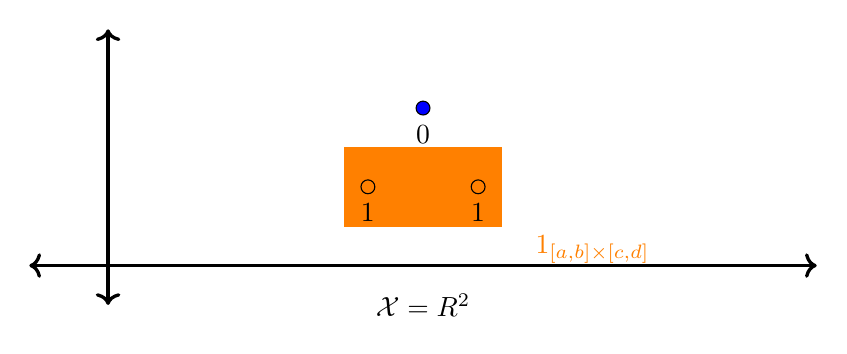
\begin{tikzpicture}
		\def\le{-1}
		\def\re{1}
		\draw[<->,very thick] (-5,0) -- (5,0);
		\draw[<->,very thick] (-4,-.5) -- (-4,3);
		\node[color=orange,below left] at (3,.5) {$1_{[a,b]\times[c,d]}$};
		\node at (0,-.5) {$\mathcal{X} = \mathbb{R}^2$} ;

		\fill[draw=black,color=orange] (-1,1.5) rectangle (1,.5);


		\node[circle,draw=black, fill=orange, inner sep=0pt,minimum size=5pt, label=below:1] at (-.7,1) {};
		\node[circle,draw=black, fill=blue, inner sep=0pt,minimum size=5pt, label=below:0] at (0,2) {};
		\node[circle,draw=black, fill=orange, inner sep=0pt,minimum size=5pt, label=below:1] at (.7,1) {};
	\end{tikzpicture}
  \end{minipage}
  \vfill
  \begin{minipage}[t][0.5\textheight][t]{\textwidth}
\textbf{Question:} What is the VC-dimension of the hypothesis class of indicator functions on the axis aligned rectangles? 

\end{minipage}
\end{frame}




\begin{frame}<handout:0>[fragile]{VC-Dimension}
  \begin{minipage}[t][0.5\textheight][t]{\textwidth}
	\centering
	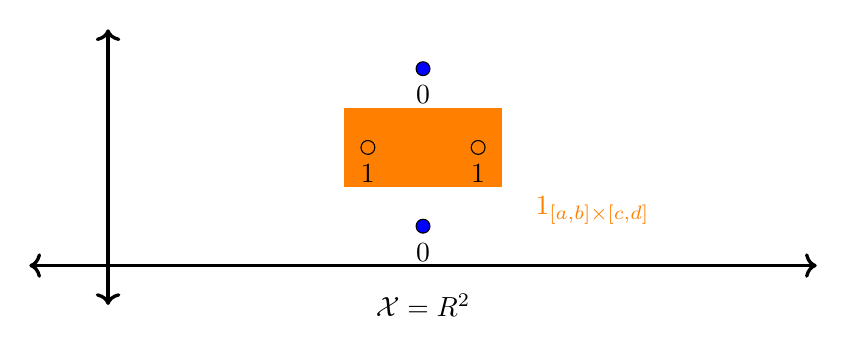
\begin{tikzpicture}
		\def\le{-1}
		\def\re{1}
		\draw[<->,very thick] (-5,0) -- (5,0);
		\draw[<->,very thick] (-4,-.5) -- (-4,3);
		\node[color=orange,below left] at (3,1) {$1_{[a,b]\times[c,d]}$};
		\node at (0,-.5) {$\mathcal{X} = \mathbb{R}^2$} ;

		\fill[draw=black,color=orange] (-1,2) rectangle (1,1);


		\node[circle,draw=black, fill=orange, inner sep=0pt,minimum size=5pt, label=below:1] at (-.7,1.5) {};
		\node[circle,draw=black, fill=blue, inner sep=0pt,minimum size=5pt, label=below:0] at (0,2.5) {};
		\node[circle,draw=black, fill=blue, inner sep=0pt,minimum size=5pt, label=below:0] at (0,.5) {};
		\node[circle,draw=black, fill=orange, inner sep=0pt,minimum size=5pt, label=below:1] at (.7,1.5) {};
	\end{tikzpicture}
  \end{minipage}
  \vfill
  \begin{minipage}[t][0.5\textheight][t]{\textwidth}
\textbf{Question:} What is the VC-dimension of the hypothesis class of indicator functions on the axis aligned rectangles? Its not hard to see that a 4 point see can be shattered.

\end{minipage}
\end{frame}




\begin{frame}<handout:0>[fragile]{VC-Dimension}
  \begin{minipage}[t][0.5\textheight][t]{\textwidth}
	\centering
	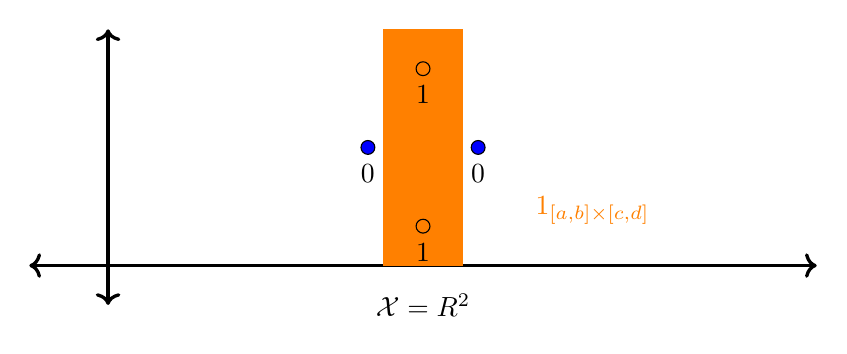
\begin{tikzpicture}
		\def\le{-1}
		\def\re{1}
		\draw[<->,very thick] (-5,0) -- (5,0);
		\draw[<->,very thick] (-4,-.5) -- (-4,3);
		\node[color=orange,below left] at (3,1) {$1_{[a,b]\times[c,d]}$};
		\node at (0,-.5) {$\mathcal{X} = \mathbb{R}^2$} ;

		\fill[draw=black,color=orange] (-.5,3) rectangle (.5,0);


		\node[circle,draw=black, fill=blue, inner sep=0pt,minimum size=5pt, label=below:0] at (-.7,1.5) {};
		\node[circle,draw=black, fill=orange, inner sep=0pt,minimum size=5pt, label=below:1] at (0,2.5) {};
		\node[circle,draw=black, fill=orange, inner sep=0pt,minimum size=5pt, label=below:1] at (0,.5) {};
		\node[circle,draw=black, fill=blue, inner sep=0pt,minimum size=5pt, label=below:0] at (.7,1.5) {};
	\end{tikzpicture}
  \end{minipage}
  \vfill
  \begin{minipage}[t][0.5\textheight][t]{\textwidth}
\textbf{Question:} What is the VC-dimension of the hypothesis class of indicator functions on the axis aligned rectangles? Its not hard to see that a 4 point see can be shattered.

\end{minipage}
\end{frame}




\begin{frame}<handout:0>[fragile]{VC-Dimension}
  \begin{minipage}[t][0.5\textheight][t]{\textwidth}
	\centering
	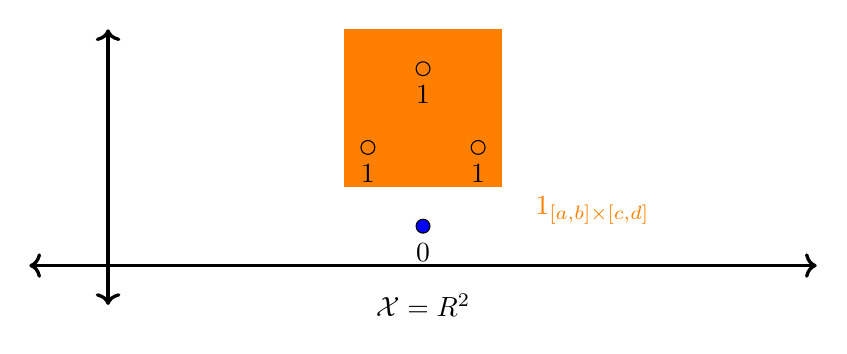
\begin{tikzpicture}
		\def\le{-1}
		\def\re{1}
		\draw[<->,very thick] (-5,0) -- (5,0);
		\draw[<->,very thick] (-4,-.5) -- (-4,3);
		\node[color=orange,below left] at (3,1) {$1_{[a,b]\times[c,d]}$};
		\node at (0,-.5) {$\mathcal{X} = \mathbb{R}^2$} ;

		\fill[draw=black,color=orange] (-1,3) rectangle (1,1);


		\node[circle,draw=black, fill=orange, inner sep=0pt,minimum size=5pt, label=below:1] at (-.7,1.5) {};
		\node[circle,draw=black, fill=orange, inner sep=0pt,minimum size=5pt, label=below:1] at (0,2.5) {};
		\node[circle,draw=black, fill=blue, inner sep=0pt,minimum size=5pt, label=below:0] at (0,.5) {};
		\node[circle,draw=black, fill=orange, inner sep=0pt,minimum size=5pt, label=below:1] at (.7,1.5) {};
	\end{tikzpicture}
  \end{minipage}
  \vfill
  \begin{minipage}[t][0.5\textheight][t]{\textwidth}
\textbf{Question:} What is the VC-dimension of the hypothesis class of indicator functions on the axis aligned rectangles? Its not hard to see that a 4 point see can be shattered.

\end{minipage}
\end{frame}



\begin{frame}<handout:0>[fragile]{VC-Dimension}
  \begin{minipage}[t][0.5\textheight][t]{\textwidth}
	\centering
	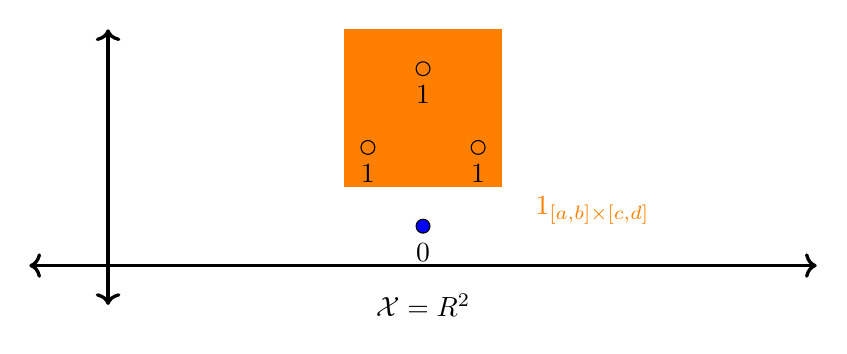
\begin{tikzpicture}
		\def\le{-1}
		\def\re{1}
		\draw[<->,very thick] (-5,0) -- (5,0);
		\draw[<->,very thick] (-4,-.5) -- (-4,3);
		\node[color=orange,below left] at (3,1) {$1_{[a,b]\times[c,d]}$};
		\node at (0,-.5) {$\mathcal{X} = \mathbb{R}^2$} ;

		\fill[draw=black,color=orange] (-1,3) rectangle (1,1);


		\node[circle,draw=black, fill=orange, inner sep=0pt,minimum size=5pt, label=below:1] at (-.7,1.5) {};
		\node[circle,draw=black, fill=orange, inner sep=0pt,minimum size=5pt, label=below:1] at (0,2.5) {};
		\node[circle,draw=black, fill=blue, inner sep=0pt,minimum size=5pt, label=below:0] at (0,.5) {};
		\node[circle,draw=black, fill=orange, inner sep=0pt,minimum size=5pt, label=below:1] at (.7,1.5) {};
	\end{tikzpicture}
  \end{minipage}
  \vfill
  \begin{minipage}[t][0.5\textheight][t]{\textwidth}
\textbf{Question:} What is the VC-dimension of the hypothesis class of indicator functions on the axis aligned rectangles? Its not hard to see that a 4 point see can be shattered. And it turns out there is no way to shatter any 5 point set. (\textbf{exercise}). 

\end{minipage}
\end{frame}







\begin{frame}[fragile]{VC-Dimension}
  \begin{minipage}[t][0.5\textheight][t]{\textwidth}
	\centering
	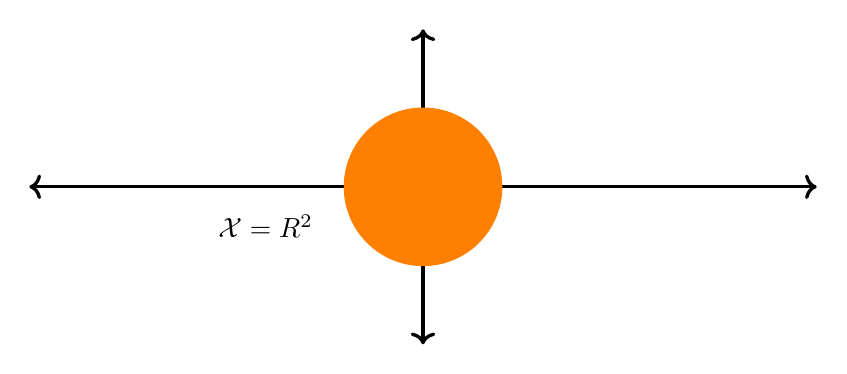
\begin{tikzpicture}
		\def\le{-1}
		\def\re{1}
		\draw[<->,very thick] (-5,0) -- (5,0);
		\draw[<->,very thick] (0,-2) -- (0,2);

		\fill[draw=black,color=orange] (0,0) circle (1);
		\node at (-2,-.5) {$\mathcal{X} = \mathbb{R}^2$};

	\end{tikzpicture}
  \end{minipage}
  \vfill
  \begin{minipage}[t][0.5\textheight][t]{\textwidth}
\textbf{Question:} What is the VC-dimension of the hypothesis class of indicator functions on the circles of radius $r\in \mathbb{R}^+$ centered at $(0,0)$? (\textbf{exercise}). 

\end{minipage}
\end{frame}










\begin{frame}[fragile]{VC-Dimension}
  \begin{minipage}[t][0.5\textheight][t]{\textwidth}
	\centering \includegraphics[height=0.6\textheight]{L6KNN.png} 
  \end{minipage}
  \vfill
  \begin{minipage}[t][0.5\textheight][t]{\textwidth}
\textbf{Question:} What is the VC-Dimension of $k$-nearest neighbors?

\end{minipage}
\end{frame}





\begin{frame}<handout:0>[fragile]{VC-Dimension}
  \begin{minipage}[t][0.5\textheight][t]{\textwidth}
	\centering \includegraphics[height=0.6\textheight]{L6KNN.png} 
  \end{minipage}
  \vfill
  \begin{minipage}[t][0.5\textheight][t]{\textwidth}
\textbf{Question:} What is the VC-Dimension of $k$-nearest neighbors? 

With a little bit of thought, its clear that 1 nearest neighbors has infinite VC dimension, since when restricted to any finite set of size $N$, it is clearly the set of all functions. What about for higher $k$?

\end{minipage}
\end{frame}






\begin{frame}[fragile]{VC-Dimension and the number of parameters}
  \begin{minipage}[t][0.5\textheight][t]{\textwidth}
	\centering
	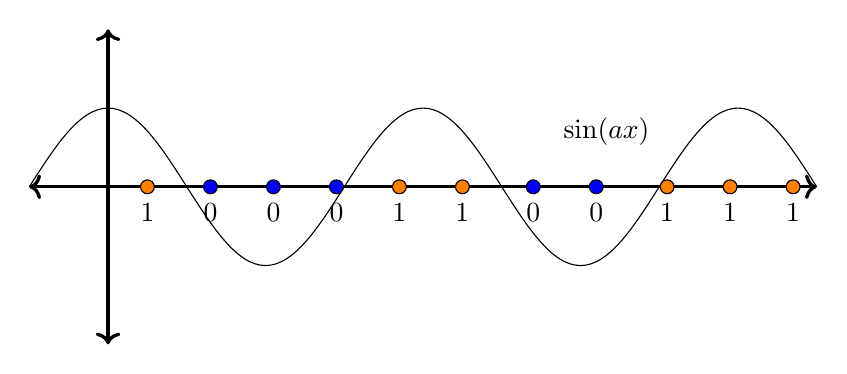
\begin{tikzpicture}
		\def\le{-1}
		\def\re{1}
		\draw[<->,very thick] (-5,0) -- (5,0);
		\draw[<->,very thick] (-4,-2) -- (-4,2);
		\node[below left] at (3,1) {$\sin(ax)$};


%		\draw (0,0) sin (1,1) cos (2,0) sin (3,-1) cos (4,0) sin (5,1) cos (6,0);
		\draw (-5,0) sin (-4,1) cos (-3,0) sin (-2,-1) cos (-1,0) sin (0,1) cos (1,0) sin (2,-1) cos (3,0) sin (4,1) cos (5,0);

		\node[circle,draw=black, fill=orange, inner sep=0pt,minimum size=5pt, label=below:1] at (-3.5,0) {};
		\node[circle,draw=black, fill=blue, inner sep=0pt,minimum size=5pt, label=below:0] at (-2.7,0) {};
		\node[circle,draw=black, fill=blue, inner sep=0pt,minimum size=5pt, label=below:0] at (-1.9,0) {};
		\node[circle,draw=black, fill=blue, inner sep=0pt,minimum size=5pt, label=below:0] at (-1.1,0) {};
		\node[circle,draw=black, fill=orange, inner sep=0pt,minimum size=5pt, label=below:1] at (-.3,0) {};
		\node[circle,draw=black, fill=orange, inner sep=0pt,minimum size=5pt, label=below:1] at (.5,0) {};
		\node[circle,draw=black, fill=blue, inner sep=0pt,minimum size=5pt, label=below:0] at (1.4,0) {};
		\node[circle,draw=black, fill=blue, inner sep=0pt,minimum size=5pt, label=below:0] at (2.2,0) {};
		\node[circle,draw=black, fill=orange, inner sep=0pt,minimum size=5pt, label=below:1] at (3.1,0) {};
		\node[circle,draw=black, fill=orange, inner sep=0pt,minimum size=5pt, label=below:1] at (3.9,0) {};
		\node[circle,draw=black, fill=orange, inner sep=0pt,minimum size=5pt, label=below:1] at (4.7,0) {};
	\end{tikzpicture}
  \end{minipage}
  \vfill
  \begin{minipage}[t][0.5\textheight][t]{\textwidth}
\textbf{Be aware:} VCDim doesn't directly measure the number of parameters, but instead some ``effective" number of parameters. \pause For example, the classifier 
$$
\text{ceil}\big[\,\sin(ax)\,\big]
$$
depends on only 1 parameter, but has infinite VC dimension.


\end{minipage}
\end{frame}





\section{The Fundamental Theorem of PAC Learning}

\begin{frame}[fragile]{Fundamental Theorem}
With the concept of VC dimension, we are finally in the position to state the theorem which will tie all of PAC learning together.
\end{frame}


\begin{frame}[fragile]{Fundamental Theorem}
\textbf{Fundamental Theorem of Statistical Learning:} Let $\cH$ be a hypothesis class of functions from a domain $\cX$ to $\{0,1\}$ and let the loss function be 0-1 loss. Then the following are equivalent:\pause
\begin{enumerate}[a)]
\item $\cH$ has the uniform convergence property. \pause
\item Any ERM rule is a successful APAC learner for $\cH$.\pause
\item $\cH$ is APAC learnable.\pause
\item $\cH$ is PAC learnable.\pause
\item Any ERM rule is a successful PAC learner for $\cH$.\pause
\item The VC-dimension of $\cH$ is finite. \pause
\end{enumerate}
We have already shown $a\to b\to c\to d\to e\to f$, it only remains to show $f\to a$. 
\end{frame}






\begin{frame}[fragile]{Fundamental Theorem: Proof Outline}
The proof is based on two main claims:\newline\pause

\textbf{(1)} First, if VCdim$(\cH) = d$, then when restricting to finite sets the ``effective size" of $\cH$ is $O(|C|^d)$. That is, the size of $\cH$ grows polynomially, not the exponential $2^{|C|}$ we might expect. This claim is known as Sauers Lemma.\pause\newline

\textbf{(2)} The second step is to show that if $|\cH_C|$ has a small ``effective size" then it enjoys the uniform convergence property. This is a very instructive but straightforward application of the standard probability inequity theorems like Markov and Hoeffding's. It it well worth studying, but is perhaps a better example of probability theory then machine learning. 
\end{frame}




\section{Sauers Lemma}


\begin{frame}[fragile]{Growth Function}
Let $\cH$ be a hypothesis class and let $\cH_{C}$ be the restriction of the functions in $\cH$ to a set $C\subseteq \cX$.. Then, the growth function of $\cH$, denoted $\tau_\cH:\bN\to\bN$ is
$$
\tau_\cH(N) = \max_{C\subset\cX\,:\, |C| = N}|\cH_{C}|\,,
$$
that is the maximum of the number of functions from $C$ to $\{0,1\}$ over all sets of size $N$. 

If $N\leq \text{VCdim}(\cH)$, than clearly $\tau_\cH(N) = 2^N$. The surprising thing is that when $N> d$, $\tau_\cH$ settles down and becomes polynomial in $N$.


\end{frame}




\begin{frame}[fragile]{Growth Function}
\textbf{Sauer (-Shelah-Perles) Lemma:} Let $\cH$ be a hypothesis class with VCdim($\cH)\leq d<\infty$. Then, for all $N$,
$$
\tau_\cH(N)\leq \sum_{i=0}^d\binom{N}{i} = \sum_{i=0}^d \frac{N!}{i!(N-i)!}\,.
$$\pause
In particular, if $N>d+1$, then 
$$
\tau_\cH(N) \leq (eN/d)^d\,,
$$
where $e = \exp(1)$. \pause

So for $N$ large enough, the effective growth of the hypothesis class over a test set is polynomial in $N$ 

\end{frame}






\begin{frame}[fragile]{Fundamental Theorem}
\textbf{Fundamental Theorem of Statistical Learning: Quantitative} Let $\cH$ be a hypothesis class of functions from a domain $\cX$ to $\{0,1\}$ with VC-dim $d$ and let the loss function be 0-1 loss. \pause Then there are absolute constants $c_1$ and $c_2$ such that

\textbf{(1)} The class $\cH$ has the uniform convergence property and is APAC learnable, with
$$
c_1 \frac{d + \log (1/\delta)}{\epsilon^2} \leq N^{UC}_\cH(\epsilon,\delta), N^{APAC}_\cH(\epsilon,\delta) \leq c_2 \frac{d + \log (1/\delta)}{\epsilon^2}\,.
$$\pause
\textbf{(2)} The class $\cH$ is PAC learnable with 
$$
c_1 \frac{d + \log (1/\delta)}{\epsilon} \leq N_\cH(\epsilon,\delta) \leq c_2 \frac{d \log(1/\epsilon)+ \log (1/\delta)}{\epsilon}\,.
$$\pause
So the VC dimension, if it can be computed, give us the asymptotic growth of the sample complexity in terms of the accuracy and precision.
\end{frame}



\begin{frame}[fragile]{Fundamental Theorem}
\textbf{Fundamental Theorem of Statistical Learning: Quantitative} Let $\cH$ be a hypothesis class of functions from a domain $\cX$ to $\{0,1\}$ with VC-dim $d$ and let the loss function be 0-1 loss. \pause Then there are absolute constants $c_1$ and $c_2$ such that

\textbf{(1)} The class $\cH$ has the uniform convergence property and is APAC learnable, with
$$
c_1 \frac{d + \log (1/\delta)}{\epsilon^2} \leq N^{UC}_\cH(\epsilon,\delta), N^{APAC}_\cH(\epsilon,\delta) \leq c_2 \frac{d + \log (1/\delta)}{\epsilon^2}\,.
$$\pause
\textbf{(2)} The class $\cH$ is PAC learnable with 
$$
c_1 \frac{d + \log (1/\delta)}{\epsilon} \leq N_\cH(\epsilon,\delta) \leq c_2 \frac{d \log(1/\epsilon)+ \log (1/\delta)}{\epsilon}\,.
$$\pause
\textbf{Note:} If $\cH$ is realizable accuracy is much cheaper, but still more expensive than precision. 
\end{frame}




\section{Boosting and PAC learning}





\begin{frame}[fragile]{Weak Learnability}
A learning algorithm $A$ is a $\gamma$-\textbf{weak learner} for a class $\cH$ if instead of forcing the true error of $A(\cT)$ less than $\epsilon$ it can instead force it less than $1/2-\gamma$. \pause 

Formally, $A$ is a $\gamma$-\textbf{weak learner} if  there exists $N:(0,1)\to \bN$ such that for every $\delta \in (0,1)$ and every distribution $\cD$ over $\cX$ and for every labeling function $f:\cX\to\{\pm 1\}$, if realizability holds then if the number of training samples $|\cT|>N(\delta)$, 
$$
L_{(\cD,f)}[\,A(\cT)\,]\leq \frac12 - \gamma \hspace{2em} \text{with probability } 1-\delta\,.
$$\pause
A hypothesis class is $\gamma$-\textbf{weak learnable} if such an algorithm exists. We call traditional PAC learnability \textbf{strong learnability}.
\end{frame}


\begin{frame}[fragile]{Weak Learnability}
Strong learnability implies that with enough data we can find arbitrary good solutions in the realizable case, while weak learnability only guarantees that we can find a learner that does better than a coin toss. \pause 

Note that the by Fundamental Theorem of Learning if $\cH$ has VC dimension $d$, then 
$$
N(\epsilon,\delta)\geq c_1\frac{d + \log(1/\delta)}{\epsilon}\,.
$$
If $\epsilon = 1/2 - \gamma$, we see that if $d=\infty$ than $\cH$ is not $\gamma$-weak learnable. Therefore ignoring computational considerations, both types of learnability are characterize by the VC dimension and so weak learning is just as ``hard'' as strong learning. \pause However, algorithms that satisfy weak learning may be much for computationally achievable. 
\end{frame}


\begin{frame}[fragile]{Adaboost Is An Efficient Learner}
\textbf{(UML Theorem 10.2)} Let $S$ be a training set and assume that at each iteration $m$ of Adaboost the weak learner returns a hypothesis for which $\epsilon_m\leq 1/2-\gamma$. \pause If $T$ classifiers are used, the training error of the output $\hat{G}(x)$ is bounded by
$$
L_{\cT}(\hat{G}) = \frac{1}{N}\sum_{i=1}^N \mathds{1}(\hat{G}(x_i)\neq y_i) \leq \exp(-2\gamma^2T)\,.
$$\pause

\textbf{Proof Sketch:} The proof rests on two ideas: Writing 
$$
Z_m = \frac{1}{N}\sum_{i=1}^N e^{-y_i f^{(m)}(x_i)}\,,
$$\pause
and noticing that $\mathds{1}(\hat{G}(x_i)\neq y_i) \leq e^{-\hat{G}(x_i) y_i}$, we can bound 
$$
L_{\cT}(\hat{G}) \leq Z_{M} = \frac{Z_M}{Z_{M-1}} \frac{Z_{M-1}}{Z_{M-2}}\cdots \frac{Z_1}{Z_{0}} \,.
$$\pause
The final step is to show $Z_m/Z_{m-1} \leq e^{-2\gamma^2}$, which is a straightward if tedious computation. \hfill $\Box$
\end{frame}




\begin{frame}[fragile]{Decision Stumps}
Each iteration of Adaboost involves $O(M)$ operations, as well as a call to the weak learner. Lets take a moment to highlight a hypothesis class that we will consider computationally efficient.\pause

The hypothesis class of decision stumps on $\bR^p$ is
$$
\cH_{DS} = \big\{\,\text{sign}(x-\theta)\cdot b\,:\,\theta\in \bR,\, i\in [p],\,b\in {\pm1}\big\}\,.
$$
It can be shown that $\cH_{DS}$ is a $\gamma = 1/12$-weak learnable in $O(pN)$ time, where $N$ is the number of samples in the training set. Therefore, the boosted hypothesis class can be learned in $O(pNM)$ time. \pause

As a comparison example, the computational complexity of least squares linear regression is $O(p^2N)$ and decision tree with depth $d$ $O(Npd)$, or between $O(Np\log N)$ and $O(N^2p)$ if $d$ is not specified. 
\end{frame}




\begin{frame}[fragile]{Weak Learnability}
  \begin{minipage}[t][0.5\textheight][t]{\textwidth}
	\centering \includegraphics[height=.5\textheight]{L19DecStump.png}\hspace{1em}\includegraphics[height=.5\textheight]{L19DecStump1.png} 
  \end{minipage}
  \vfill
\begin{minipage}[t][0.5\textheight][t]{\textwidth}
Boosting will clearly increase the VD dimension, but it does so in a controlled way. 

\textbf{Questions:} The VC dimension of the 1d decision stump is 2. What is the VC dimension of the $M$ boosted 1d decision stump?
\end{minipage}
\end{frame}




\begin{frame}[fragile]{The Boosted VC dimension}
The VC dimension of a linear combination of $M$ classifiers is upper bounded in terms of the $M$ and the VC dimension of the base class:\pause

\textbf{(UML Lemma 10.3)} Let $B$ be a basis of functions with fixed VC dimension $d_B$ and let $L(B,M)$ be the sign of a weighted sum of elements of $B$. Assume that $M$ and $d_B$ are larger than 3. Then 
$$
\text{VDdim}(L(B,T)) \leq M(d_B + 1)(3\log(M(d_B+1))+2)\,.
$$\pause

This tells us more or less exactly how the VC dimension changes as we boost a weak learner. Ignoring the logarithmic terms, the VC dimension of the boosted learner grows like $M(d_B + 1)$. The parameter $M$ gives us granular control over the bias variance tradeoff at both a theoretical and computational complexity level. 
\end{frame}




\section{VC-Dimension and Neural Networks}


\begin{frame}[fragile]{VC dimension of ANNs}
Finally, let us discuss the sample complexity of artificial neural networks. We will need a lemma:\pause

\textbf{Lemma:} Assume the hypothesis class $\cH$ is form by the composition of hypothesis classes $\cH_j$, that is for all $h\in \cH$,
$$
h = h_L\circ\ldots \circ h_1,\,\,\,\,\text{for } h_i\in \cH_j\,.
$$
Then the growth function $\tau_\cH$ is bounded by the products of the growth functions $\tau_{\cH_j}$:
$$
\tau_\cH(N) \leq \prod_{j=1}^L \tau_{\cH_j}(N)
$$
 (\textbf{Proof: HW 3, Question 3}).

\end{frame}





\begin{frame}[fragile]{VC dimension of ANNs}
\begin{minipage}[t][0.5\textheight][t]{\textwidth}\centering
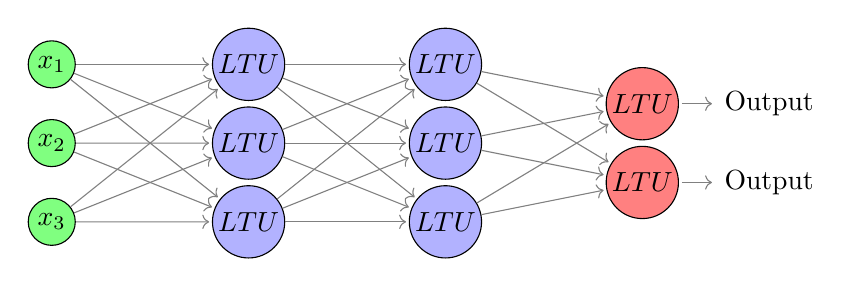
\begin{tikzpicture}[shorten >=1pt,->,draw=black!50, node distance=\layersep]
    \tikzstyle{every pin edge}=[<-,shorten <=1pt]
    \tikzstyle{neuron}=[circle,fill=black!25,minimum size=17pt,inner sep=0pt, draw=black]
    \tikzstyle{input neuron}=[neuron, fill=green!50];
    \tikzstyle{output neuron}=[neuron, fill=red!50];
    \tikzstyle{hidden neuron}=[neuron, fill=blue!30];
    \tikzstyle{annot} = [text width=4em, text centered]

    % Draw the input layer nodes
    \foreach \name / \y in {1,...,3}
    % This is the same as writing \foreach \name / \y in {1/1,2/2,3/3,4/4}
        \node[input neuron] (I-\name) at (0,-\y) {$x_\y$};

    % Draw the hidden layer nodes
    \foreach \name / \y in {1,...,3}
        \path[yshift=0cm]
            node[hidden neuron] (H1-\name) at (\layersep,-\y cm) {$\, LTU\, $};

    % Draw the hidden layer nodes
    \foreach \name / \y in {1,...,3}
        \path[yshift=0cm]
            node[hidden neuron] (H2-\name) at (\layersep + \layersep,-\y cm) {$\, LTU\, $};


    % Draw the output layer node
    \foreach \name / \y in {1,...,2}
    		\node[output neuron,pin={[pin edge={->}]right:Output}] (O-\y) at (\layersep + \layersep + \layersep,-\y cm-.5cm) {$\,LTU\,$};

    % Connect every node in the input layer with every node in the
    % hidden layer.
    \foreach \source in {1,...,3}
        \foreach \dest in {1,...,3}
            \draw (I-\source) --  (H1-\dest);

    % Connect every node in the input layer with every node in the
    % hidden layer.
    \foreach \source in {1,...,3}
        \foreach \dest in {1,...,3}
            \draw (H1-\source) --  (H2-\dest);


    % Connect every node in the hidden layer with the output layer
    \foreach \source in {1,...,3}
		\foreach \dest in {1,...,2}
        		\path (H2-\source) edge (O-\dest);
\end{tikzpicture}
  \end{minipage}
  \vfill
\begin{minipage}[t][0.5\textheight][t]{\textwidth}
Let $\cH$ be the hypothesis class of multilayer perceptron networks with $L$ layers, each with $N_j$ nodes, and with $\sigma(z) = \text{sign}(z)$. We can express $\cH$ as a composition of hypothesis classes $\cH_j$, where each $h_j\in \cH_j$ is a function $h:\mathbb{R}^{N_j}\to\{\pm1\}$.
\end{minipage}
\end{frame}





\begin{frame}[fragile]{VC dimension of ANNs}
\begin{minipage}[t][0.5\textheight][t]{\textwidth}\centering
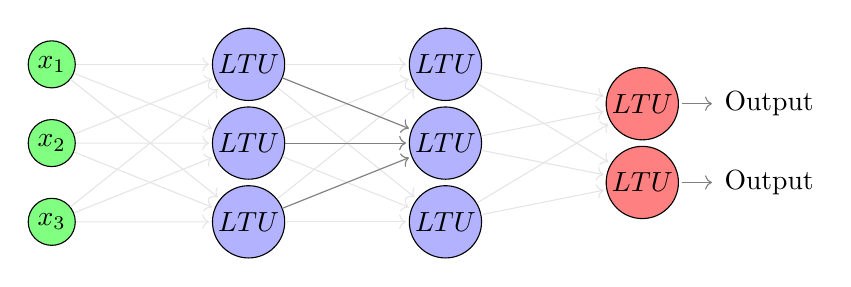
\begin{tikzpicture}[shorten >=1pt,->,draw=black!50, node distance=\layersep]
    \tikzstyle{every pin edge}=[<-,shorten <=1pt]
    \tikzstyle{neuron}=[circle,fill=black!25,minimum size=17pt,inner sep=0pt, draw=black]
    \tikzstyle{input neuron}=[neuron, fill=green!50];
    \tikzstyle{output neuron}=[neuron, fill=red!50];
    \tikzstyle{hidden neuron}=[neuron, fill=blue!30];
    \tikzstyle{annot} = [text width=4em, text centered]

    % Draw the input layer nodes
    \foreach \name / \y in {1,...,3}
    % This is the same as writing \foreach \name / \y in {1/1,2/2,3/3,4/4}
        \node[input neuron] (I-\name) at (0,-\y) {$x_\y$};

    % Draw the hidden layer nodes
    \foreach \name / \y in {1,...,3}
        \path[yshift=0cm]
            node[hidden neuron] (H1-\name) at (\layersep,-\y cm) {$\, LTU\, $};

    % Draw the hidden layer nodes
    \foreach \name / \y in {1,...,3}
        \path[yshift=0cm]
            node[hidden neuron] (H2-\name) at (\layersep + \layersep,-\y cm) {$\, LTU\, $};


    % Draw the output layer node
    \foreach \name / \y in {1,...,2}
    		\node[output neuron,pin={[pin edge={->}]right:Output}] (O-\y) at (\layersep + \layersep + \layersep,-\y cm-.5cm) {$\,LTU\,$};

    % Connect every node in the input layer with every node in the
    % hidden layer.
    \foreach \source in {1,...,3}
        \foreach \dest in {1,...,3}
            \draw[draw=gray!20] (I-\source) --  (H1-\dest);

    % Connect every node in the input layer with every node in the
    % hidden layer.
    \foreach \source in {1,...,3}
        \foreach \dest in {1,...,3}
            \draw[draw=gray!20] (H1-\source) --  (H2-\dest);
            
    \foreach \source in {1,...,3}
        \foreach \dest in {2}
            \draw[draw=gray] (H1-\source) --  (H2-\dest);


    % Connect every node in the hidden layer with the output layer
    \foreach \source in {1,...,3}
		\foreach \dest in {1,...,2}
        		\path[draw=gray!20] (H2-\source) edge (O-\dest);
\end{tikzpicture}
  \end{minipage}
  \vfill
\begin{minipage}[t][0.5\textheight][t]{\textwidth}
We can further decompose $\cH_j = \cH_{j,1}\times \ldots \times \cH_{j,N_j}$ into a Cartesian product, where each $\cH_{j,k}$ is the weighted functions from the previous layer into the $k$'th node. Furthermore, the growth function for the product of classes can be bounded by
$$
\tau_{\cH_j }(M)\leq \prod_{k}\tau_{\cH_{j,k}}\,. 
$$
\end{minipage}
\end{frame}




\begin{frame}[fragile]{VC dimension of ANNs}
Now, lets think carefully: At each layer, let $d_{j,k}$ be the number of edges terminating in the $k$'th node of layer $j$, or $d_{j,k} =  N_{k-1}+1$ if a additive bias is included. Each of these is a halfplane classifier on a space of dimension $d_{j,k}$, and so by Sauer's Lemma
$$
\tau_{\cH_{j,k}}(M)\leq \left( \frac{em}{d_{j,k}} \right)^{d_{j,k}} \leq (e M)^{d_{j,k}}\,.
$$
\pause
Putting this together, we find that 
$$
\tau_{\cH}(M)\leq (e M)^{\sum_{j,k} d_{j,k}} = (eM)^{|W|}\,,
$$
where $|W|$ is the total number of weights in the network. \pause If we want to shatter $M$ points, we need at least $2^{M}$ functions, so we can only shatter $M$ points with $\cH$ if
$$
2^M\leq (eM)^{|W|}\,,\,\,\,\,\text{or}\,\,\, M\leq |W|\log(eM)/\log(2)\,.
$$
\end{frame}



\begin{frame}[fragile]{VC dimension of ANNs}
Rearranging, 
$$
\frac{M}{\log M} \leq C |W|\,,
$$
so $M$'s growth is bounded by $|W|$. Therefore 
$$
M = \text{VCdim}(\cH)  = O(|W|\log |W|)\,.
$$
The VC dimension of a theoretical neural network grows proportional to the number of weights. 
\end{frame}




\begin{frame}[fragile]{VC dimension of ANNs}
Rearranging, 
$$
\frac{M}{\log M} \leq C |W|\,,
$$
so $M$'s growth is bounded by $|W|$. Therefore 
$$
M = \text{VCdim}(\cH)  = O(|W|\log |W|)\,.
$$
The VC dimension of a theoretical neural network grows proportional to the number of weights. 
\end{frame}


\begin{frame}[fragile]{VC dimension of ANNs}
The VC dimension is a combinatorial property of a hypothesis classes of classifiers that characteristic its  learnability under the PAC learning framework. The fundamental theorem of machine learning state that a class is PAC learnable, and so APAC learnable, if and only if the VC dimension is finite. \pause

The VC dimension exactly specifies the sample complexity required for PAC/APAC learning, however, in practice the VC dimension acts as an upper bound on learning. There are many cases, like neural networks, where strong empirical results can be found even when the amount of data is far below the sample complexity. In these cases, it is prior knowledge and a restricted domain that leads to the success of these methods. \pause

One of the biggest areas of theoretical machine learning research is in the description of sample spaces like visual classification tasks, both to reduce the dimensionality of the space both for better description, and for a better understanding of the theoretical bounds on learning these tasks.  
\end{frame}





\begin{frame}[fragile]{Reference}
Understanding Machine Learning, Chapters 6 and 20. 
\end{frame}




\end{document}








\begin{frame}[fragile]{Avoiding Underfitting}
The no free lunch theorem isn't the end of machine learning, it simply asserts that there is no universally best learner for every task. If fact, it implies that we should use any prior knowledge to avoid learners that perform poorly on a distribution. Such prior knowledge can be expressed by restricting the hypothesis class. \pause

But how do we choose this class? On one hand, we want a class that contains a classifier that will return the minimum error. On the other hand, the class of all functions is clearly not learnable so we cant just choose the richest class. 
\end{frame}



\begin{frame}[fragile]{Bias, Variance and Parameters}
  \begin{minipage}[t][0.5\textheight][t]{\textwidth}
	\centering
	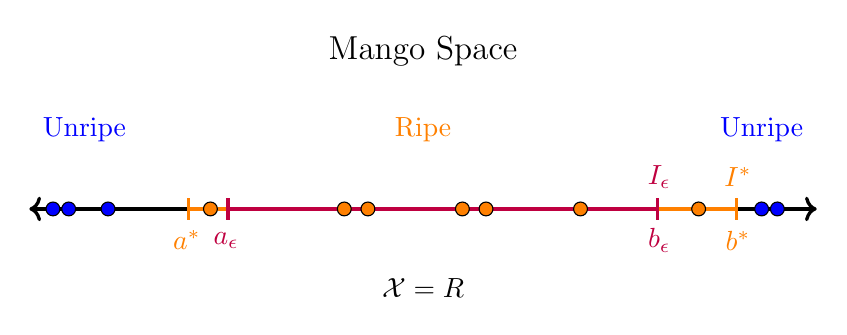
\begin{tikzpicture}
		\draw[<->,very thick] (-5,0) -- (5,0);
		\draw[color = orange, |-|,very thick] (-3,0) -- (4,0);
		\node[color=orange] at (4,.4) {$I^*$};
		\node at (0,2) {\large Mango Space} ;
		\node at (0,-1) {$\mathcal{X} = \mathbb{R}$} ;
		\node [color=blue] at (-4.3,1) {Unripe} ;
		\node [color=blue] at (4.3,1) {Unripe} ;
		\node [color=orange] at (0,1) {Ripe} ;

		\node [color=orange] at (-3,-.4) {$a^*$} ;
		\node [color=orange] at (4,-.4) {$b^*$} ;

		\draw [color=purple, |-|,very thick] (-2.5,0) -- (3,0);
		\node [color=purple] at (3,.4) {$I_\epsilon$} ;
		\node [color=purple] at (-2.5,-.4) {$a_\epsilon$} ;
		\node [color=purple] at (3,-.4) {$b_\epsilon$} ;

%		\draw [color=olive, |-|,very thick] (-3.5,0) -- (2.5,0);
%		\node [color=olive] at (3,.4) {$h_{\mathcal{T}}$} ;



		\node[circle,draw=black, fill=orange, inner sep=0pt,minimum size=5pt] at (2,0) {};
		\node[circle,draw=black, fill=orange, inner sep=0pt,minimum size=5pt] at (-1,0) {};
		\node[circle,draw=black, fill=orange, inner sep=0pt,minimum size=5pt] at (-.7,0) {};
		\node[circle,draw=black, fill=orange, inner sep=0pt,minimum size=5pt] at (.5,0) {};
		\node[circle,draw=black, fill=orange, inner sep=0pt,minimum size=5pt] at (.8,0) {};
		\node[circle,draw=black, fill=orange, inner sep=0pt,minimum size=5pt] at (-2.7,0) {};
		\node[circle,draw=black, fill=orange, inner sep=0pt,minimum size=5pt] at (3.5,0) {};

		\node[circle,draw=black, fill=blue, inner sep=0pt,minimum size=5pt] at (-4.5,0) {};
		\node[circle,draw=black, fill=blue, inner sep=0pt,minimum size=5pt] at (-4,0) {};
		\node[circle,draw=black, fill=blue, inner sep=0pt,minimum size=5pt] at (-4.7,0) {};
		\node[circle,draw=black, fill=blue, inner sep=0pt,minimum size=5pt] at (4.3,0) {};
		\node[circle,draw=black, fill=blue, inner sep=0pt,minimum size=5pt] at (4.5,0) {};
	\end{tikzpicture}
  \end{minipage}
  \vfill
  \begin{minipage}[t][0.5\textheight][t]{\textwidth}
Lets understand this visually.
$$
Err(x_0) = \sigma_\epsilon^2 + [E_\cT[\hat f(x_0)] - f(x_0)]^2 + E_\cT\big[ \hat{f}(x_0) - E_\cT[\hat{f}(x_0)] \big]^2\,.
$$\pause
Consider a data set, 
\end{minipage}
\end{frame}


\begin{frame}[fragile]{Point Variance of Linear Predictor}
Since $x_0^T  (\bfX^T\bfX)^{-1}\bfX^T\epsilon$ is a vector, squaring it is the same as multiply by its transpose. \pause This allow us to write
\begin{align*}
\action<+->{\textbf{Var} &= E_\cT\big[(\,x_0^T  (\bfX^T\bfX)^{-1}\bfX^T\epsilon\,)^2\big] && \text{From before,}}
\\
\action<+->{  &=   E_\cT\big[(\,x_0^T  (\bfX^T\bfX)^{-1}\bfX^T\epsilon\,)(\,x_0^T  (\bfX^T\bfX)^{-1}\bfX^T\epsilon\,)^T\big]  && }
\\
\action<+->{  &=   E_\cT\big[(\,x_0^T  (\bfX^T\bfX)^{-1}\bfX^T\epsilon\,)(\epsilon^T \bfX (\bfX^T\bfX)^{-1} \,x_0)\big] &&  }
\\
\action<+->{  &= (\,x_0^T  (\bfX^T\bfX)^{-1}\bfX^T) E_\cT[\epsilon\epsilon^T] (\bfX (\bfX^T\bfX)^{-1} x_0)  &&\bfX,\,x_0\,\text{const,}}
\\
\action<+->{  &=  (\,x_0^T  (\bfX^T\bfX)^{-1}\bfX^T)\,(\sigma_\epsilon^2 I)\, (\bfX (\bfX^T\bfX)^{-1} x_0)  && \text{Def. of Var,} }
\\
\action<+->{  &=  \sigma^2_\epsilon \, \,x_0^T  (\bfX^T\bfX)^{-1}x_0  && \text{Simplify.} }
\end{align*}
\action<+->{The variance is proportional to the variance in the random variable. But how do we understand the matrix $(\bfX^T\bfX)^{-1}$?}
\end{frame}


























